\documentclass{standalone}
\usepackage{tikz}
\begin{document}
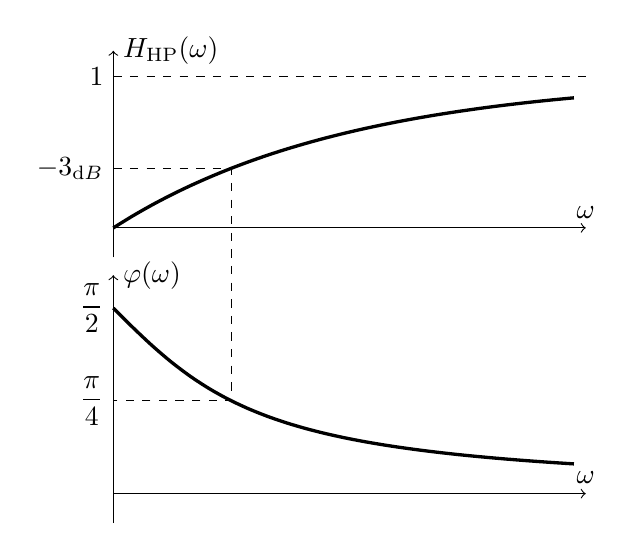
\begin{tikzpicture}[scale=1.5]
    \draw[->](0,1.75)--(0,3.5)node[right]{$H_{\mathrm{HP}}(\omega)$};
    \draw[->](0,2)--(4,2)node[above]{$\omega$};
    \draw[dashed](0,3.284)node[left]{$1$}--(4,3.284);
    \draw[very thick, smooth, domain=0:3.9]plot(\x,{3.284-e^(-0.5*(\x-0.5))});
    \draw[->](0,-0.5)--(0,1.6)node[right]{$\varphi(\omega)$};
    \node[left]at(0,1.3207){$\displaystyle\frac{\pi}{2}$};
    \draw[very thick, smooth, domain=0:3.9]plot(\x,{pi/180*atan(-\x)-0.25+pi/2});
    \draw[->](0,-0.25)--(4,-0.25)node[above]{$\omega$};
    \draw[dashed](0,2.505)node[left]{$-3_{\mathrm{d}B}$}--(1,2.505)--(1,0.535)--(0,0.535)node[left]{$\displaystyle\frac{\pi}{4}$};
\end{tikzpicture}
\end{document}